\chapter{Application and Deployment}
\label{chap:application}

\section{Integrated serving architecture}

The application operates as an \textbf{in-process model-serving modular monolith}. FastAPI imports the scoring package directly, which keeps the request path simple and avoids a separate model-serving network hop. Scored transactions are persisted through PostgreSQL or the local SQLite configuration, while the React dashboard consumes typed API responses. This arrangement is appropriate for a controlled academic demonstration because the data contract, scoring logic, persistence layer, and user interface can be exercised together; however, it also concentrates several responsibilities in one deployable unit and therefore leaves scaling, isolation, and operational fault handling for future work.

The request path begins when a transaction is submitted or imported. The API
validates the request shape, maps the available fields to the canonical
feature order, invokes the packaged model, applies calibration and policy
mapping, and persists the resulting score. The response then carries both
machine-oriented values, such as probability and model version, and
human-oriented values, such as risk band, decision, and feature explanation.
Keeping these values together makes it possible to reproduce what the analyst
saw at the time of review and to distinguish an old score from a score produced
after a model update.

\section{Scoring and review workflow}

For each scored transaction, the backend returns a calibrated probability, a risk score on a \val{0}--\val{100} scale, a risk band, an operational decision, and TreeSHAP attributions. The probability expresses the model output, whereas the risk band and decision are policy-facing interpretations and should not be confused with the learned model itself. Scored transactions and human analyst reviews are stored as distinct database entities, allowing the system to preserve both the automated assessment and the later human outcome. The interface figures in this section show how the monitoring queue, transaction detail, explanation panel, and review action form one analyst workflow.

The operating policy is explicit in the packaged V2 artifact. The review
threshold is fraud probability \val{0.16}, and the reject threshold is
\val{0.53}. The review threshold is selected by maximising recall and then F1
subject to minimum precision \val{0.30}; the reject threshold is the lowest
threshold meeting minimum reject precision \val{0.60}. After conversion to a
risk score, scores \val{0}--\val{19} are low and approve, \val{20}--\val{39}
are guarded and approve, \val{40}--\val{59} are medium and review,
\val{60}--\val{79} are high and review, and \val{80}--\val{100} are critical
and reject. This policy is separate from model ranking and can be changed
through a governed policy update without changing the learned weights.

The review workflow is designed as a human-in-the-loop process. A high-risk
score creates a prioritisation signal, not an automatic declaration of fraud.
An analyst can inspect the transaction context and the most influential
features, then record a review outcome. Separating the automated score from the
human review is valuable for later evaluation because analyst labels can be
used to examine false positives, missed fraud, and threshold performance. It
also avoids overwriting the original model output when a reviewer disagrees
with the prediction.

\begin{figure}[H]
  \centering
  \begin{subfigure}[t]{0.48\textwidth}
    \centering
    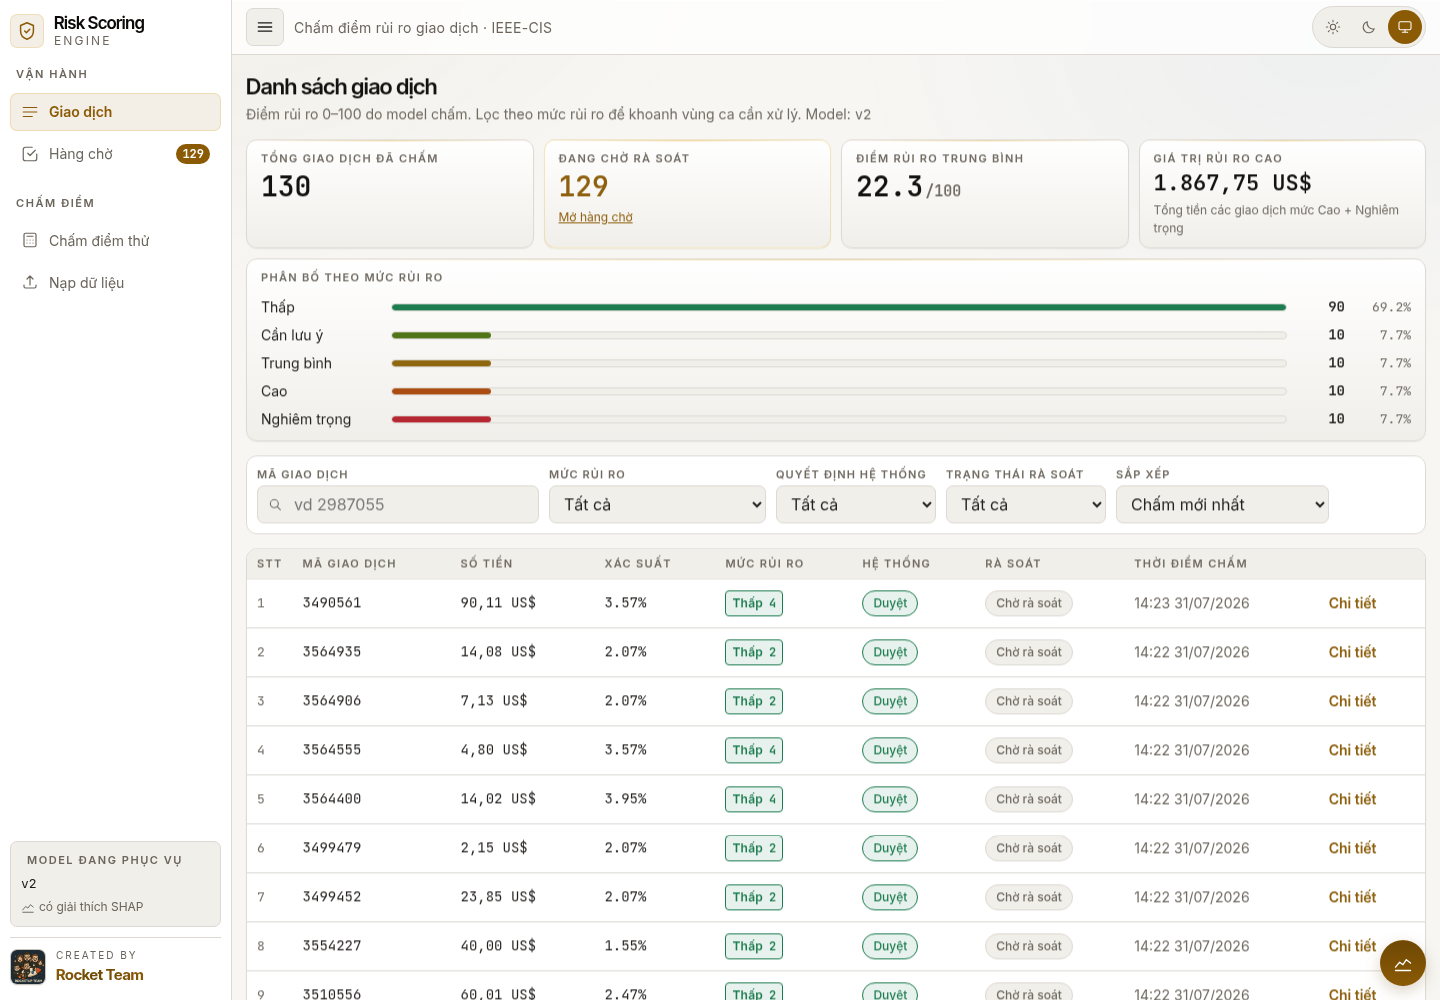
\includegraphics[width=\linewidth,height=0.38\textheight,keepaspectratio]{figures/transactions.png}
    \caption{Transaction monitoring queue.}
    \label{fig:ui-transactions}
  \end{subfigure}\hfill
  \begin{subfigure}[t]{0.48\textwidth}
    \centering
    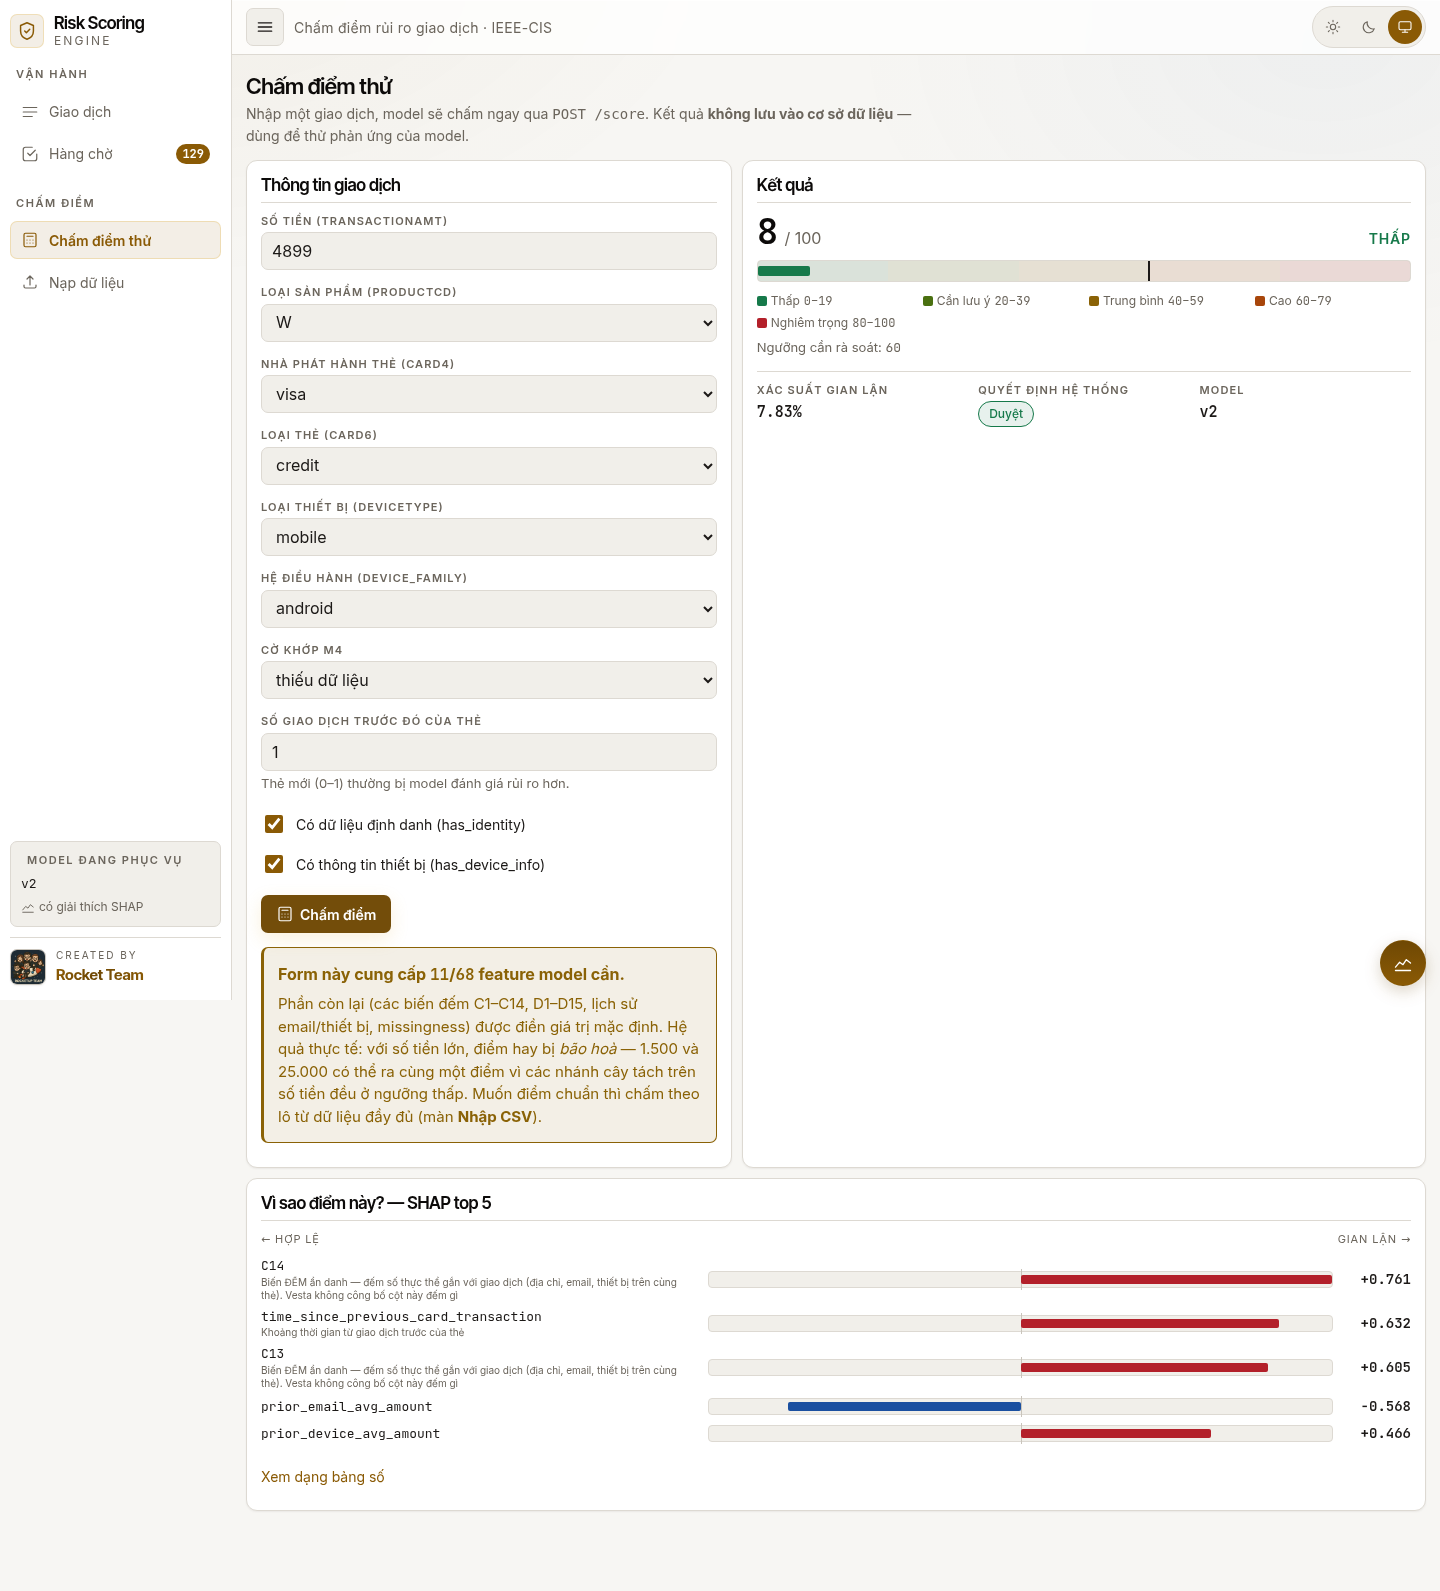
\includegraphics[width=\linewidth,height=0.38\textheight,keepaspectratio]{figures/score-result.png}
    \caption{Risk score and SHAP feature importance.}
    \label{fig:ui-score-result}
  \end{subfigure}
  \caption{Primary analyst views for triage and model-assisted risk interpretation.}
\end{figure}

\begin{figure}[H]
  \centering
  \begin{subfigure}[t]{0.48\textwidth}
    \centering
    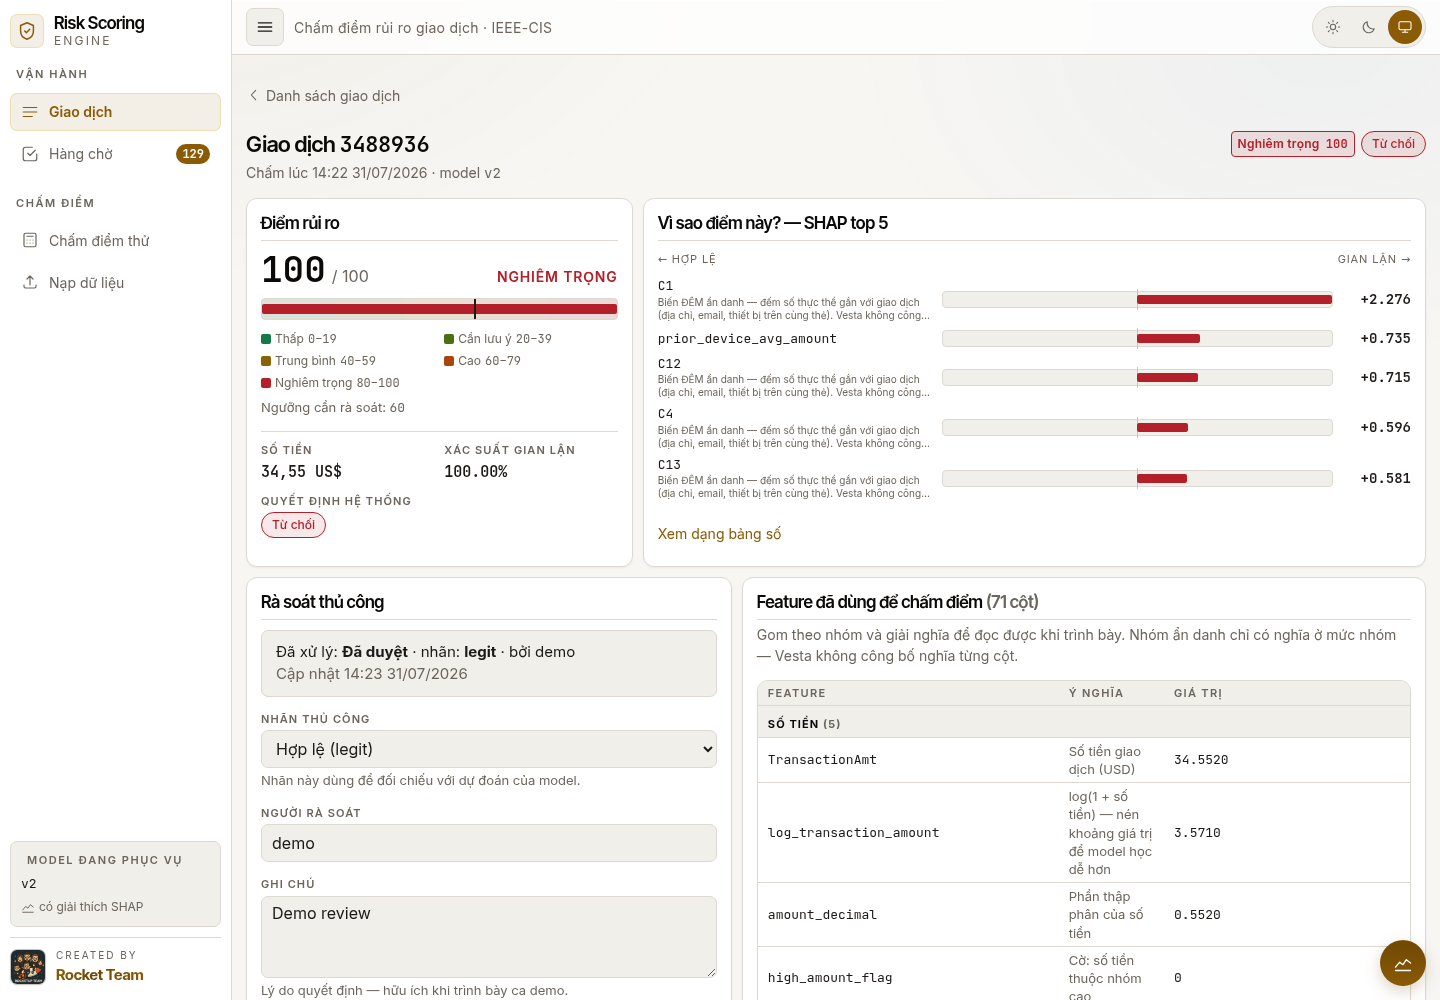
\includegraphics[width=\linewidth,height=0.38\textheight,keepaspectratio]{figures/detail.png}
    \caption{Transaction detail panel.}
    \label{fig:ui-detail}
  \end{subfigure}\hfill
  \begin{subfigure}[t]{0.48\textwidth}
    \centering
    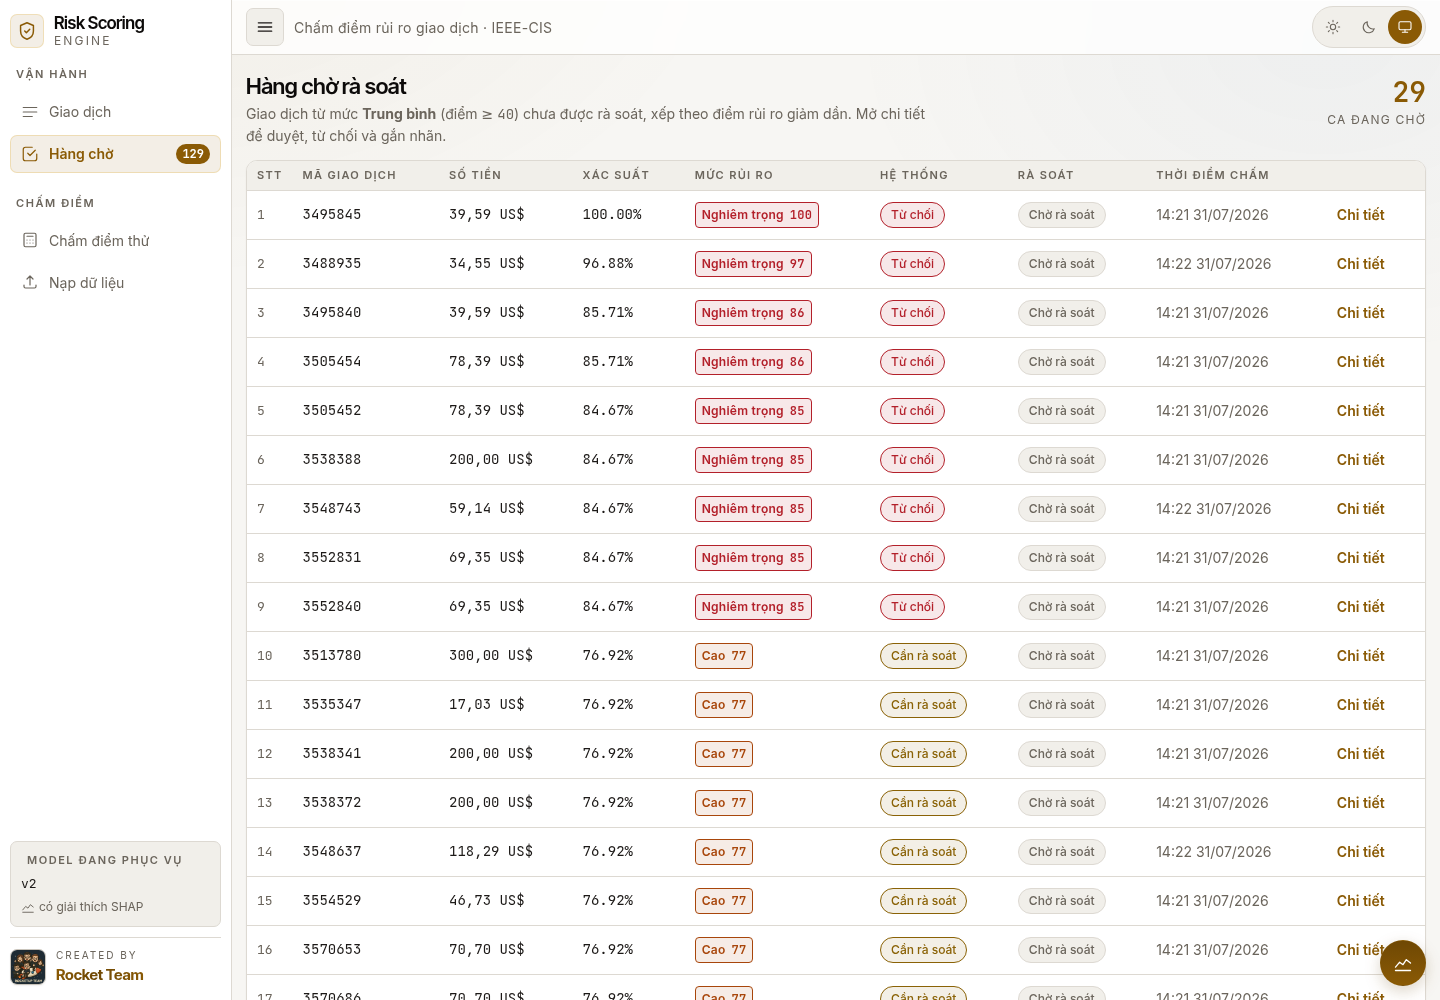
\includegraphics[width=\linewidth,height=0.38\textheight,keepaspectratio]{figures/review.png}
    \caption{Analyst fraud review workflow.}
    \label{fig:ui-review}
  \end{subfigure}
  \caption{Detailed inspection and human-review actions supported by the application.}
\end{figure}

\section{Deployment boundary}

Docker Compose orchestrates the preprocessing, training, backend, and React UI profiles, with processed Parquet artifacts mounted into the backend container. This provides a repeatable local deployment path and makes the subsystem boundaries visible to evaluators. It should not be interpreted as evidence of production availability: the current deployment still relies on local configuration, limited background-job durability, incomplete security controls, and a fallback path whose operational behaviour requires stronger monitoring.

The deployment boundary is therefore deliberately local and demonstrable. It
supports repeatable evaluation of the data contract, model package, API
responses, persistence path, and user-interface flow on one controlled
environment. It does not yet establish multi-instance coordination, durable
queue processing, secret management, service-level latency, or safe recovery
from partial failure. Those properties require an operational environment and
test evidence beyond the current academic scope.

No formal latency benchmark or throughput target is claimed in this report.
The repository includes API tests and a warm-up path for model loading, but
request-time p50/p95 latency, concurrent-request capacity, and end-to-end
batch throughput require a controlled performance test on the target hardware.
This distinction prevents the port configuration and successful functional
response from being misread as production performance evidence.
